\paragraph*{Multi-Task Imitation Learning}\mbox{}\\
The methods discussed in the previous paragraphs describe architectures and approaches specifically designed to solve a single task, with limited generalization to the object's category (e.g., picking blocks rather than balls) and initial state (e.g., the object's starting position). For instance, a system trained for pick-and-place operations cannot be repurposed for tasks like assembly operations. The methods described in this paragraph address these limitations, solving the problem of \textit{Multi-Task Imitation Learning} (MTIL)

Before starting to present and describe the different methods and approaches, it is necessary to describe the problem. Starting from a reformulation of the dataset used to train the system and the learned policy.
Indeed, in Section~\ref{sec:problem_formulation}, the expert dataset $\mathcal{D}^{E}$ has been introduced. Based on the problem to solve this dataset can composed in different way. Specifically, in the context of MTIL, the dataset $\mathcal{D}^{E}$ can be seen as a composition of $n$ datasets, $\mathcal{D}^{E}=\left \{\mathcal{D}_{1}, \dots, \mathcal{D}_{n}\right \}$, where $\mathcal{D}_{i} = \left \{ (\tau_{m_{i}}^{j}, \ c_{m_{i}}), j=1,\dots,N, \ m_{i} \in \mathcal{M}_{i}\right \}$ is the \textit{single-task dataset}, composed of:
\begin{itemize}
    \item $N$ expert demonstration for each $m^{th}$ variation of the $i^{th}$ task, where $M_{i}$ is the number of variation for the $i^{th}$ task.
    \item Agent trajectories $\tau_{m_{i}}^{j} = (s_{0}, a_{0}, s_{1}, a_{1}, \dots, a_{T-1}, s_{T})$. where $s_{t}$ is the state at time $t$ and $a_{t}$ is the corresponding action (Section \ref{sec:problem_formulation}).
    \item Task-conditioning signal $c_{m_{i}}$ for the $m^{th}$ variation of $i^{th}$ task, which describes the desired task in terms of video demonstrations \cite{james2018task_embedded,bhutani2022attentive_one_shot,dasari2021transformers_one_shot,mandi2022towards_more_generalizable_one_shot}, natural language description \cite{stepputtis2020language,jang2022bc_z,mees2022calvin,doasIcan2022,mees2022hulc,brohan2022rt,shridhar2023perceiver} or multi-modal prompt, that exploits both visual information (e.g., an image of the target object) and text information that contains the information related to the action to be performed \cite{jiang2023vima}.
\end{itemize}
The goal of Multi-Task Imitation Learning is to learn a \textit{conditioned policy} $\pi^{L}_{\theta}(a_{t}|s_{t}, c_{m_{i}})$, that is able to map the current state and command into the corresponding action.
Depending on how the policy is defined, various loss functions come into play. In the case of deterministic policies, the learning process focuses on minimizing the Mean-Squared Error (refer to Formula \ref{eq:mse}). However, for probabilistic policies, the learning process centers around minimizing the Negative Log-likelihood (refer to Formula \ref{eq:nll}). This approach aims to enhance the probability of correctly executing the action.
% \begin{equation}
%     \label{eq:mse}
%     \mathcal{L}(D^{E}, \pi^{L}_{\theta}) = \frac{1}{n} \sum_{\mathcal{D}^{i} \sim \mathcal{D}^{E}} \frac{1}{N} \sum_{(\tau_{m_{i}}^{j}, c_{m_{i}}) \sim \mathcal{D}^{i}} \frac{1}{T}\sum_{t=0}^{T} (a_{t} - \pi^{L}_{\theta}(s_{t}, c_{m_{i}}))
% \end{equation}
% \begin{equation}
%     \label{eq:nll}
%     \mathcal{L}(D^{E}, \pi^{L}_{\theta}) = \frac{1}{n} \sum_{\mathcal{D}^{i} \sim \mathcal{D}^{E}} \frac{1}{N} \sum_{(\tau_{m_{i}}^{j}, c_{m_{i}}) \sim \mathcal{D}^{i}} \frac{1}{T}\sum_{t=0}^{T} (a_{t} - \pi^{L}_{\theta}(s_{t}, c_{m_{i}}))
% \end{equation}

\begin{equation}
    \label{eq:mse}
    \mathcal{L}(\tau_{m_{i}}^{j}, c_{m_{i}},\pi^{L}_{\theta}) = \frac{1}{T}\sum_{t=0}^{T} (a_{t} - \pi^{L}_{\theta}(s_{t}, c_{m_{i}}))^{2}
\end{equation}
\begin{equation}
    \label{eq:nll}
    \mathcal{L}(\tau_{m_{i}}^{j}, c_{m_{i}},\pi^{L}_{\theta}) = - \frac{1}{T}\sum_{t=0}^{T} log(\pi^{L}_{\theta}(a_{t}|s_{t}, c_{m_{i}}))
\end{equation}
The following sections will describe the various approaches proposed to address the problem. Figure \ref{fig:mtil_taxonomy} illustrates the taxonomy used for the Multi-Task Imitation Learning methods. Specifically, the methods are categorized based on the type of generalization required by the algorithm (Few-Shot vs. Zero-Shot). For Few-Shot generalization, the Meta-Learning paradigm will be discussed, as it is most relevant to the problem at hand. For Zero-Shot generalization, the methods are further divided based on the type of conditioning signal used, whether it is provided through natural language descriptions or visual information.
\begin{figure}[t]
    \centering
    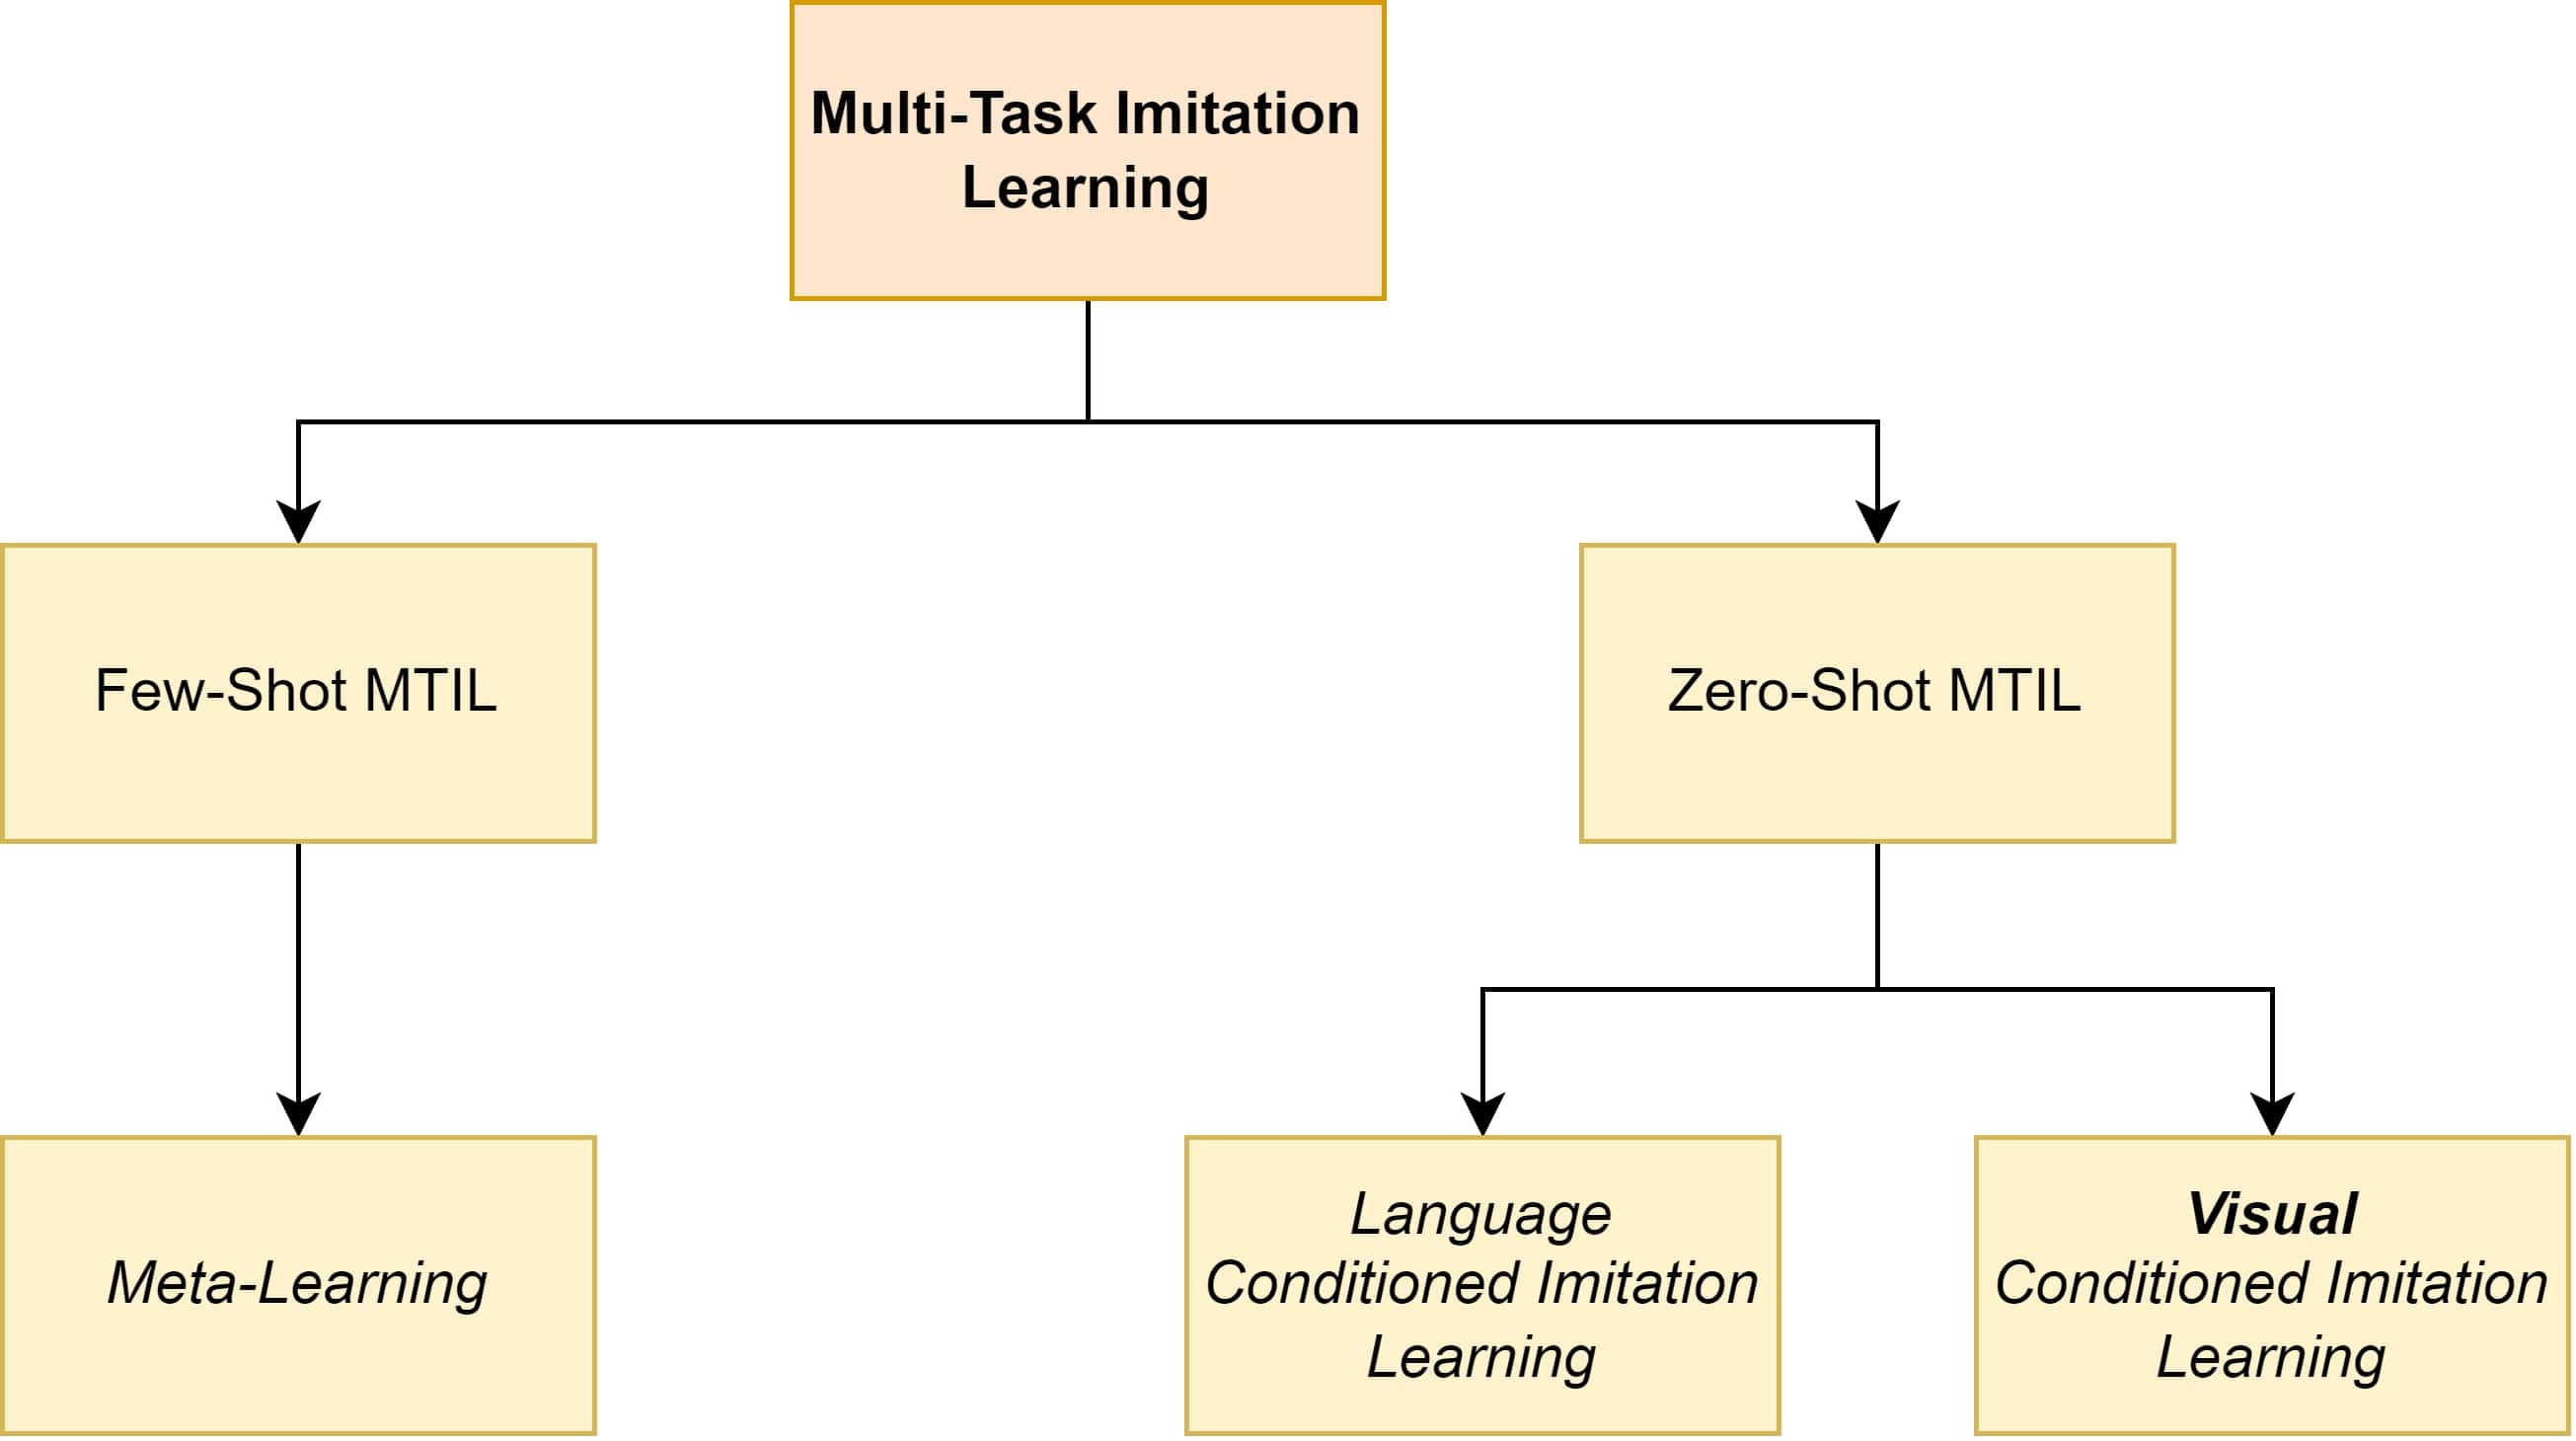
\includegraphics[width=0.8\textwidth]{figures/images/MTIL_taxonomy.jpg}
    \caption{Multi-Task Imitation Learning Taxonomy.}
    \label{fig:mtil_taxonomy}
    
\end{figure}


\textbf{Few-Shot MTIL} refers to approaches designed to train a model on a variety of tasks so that it can effectively solve a new task using only a small number of samples and consequently requires only a few back-propagation steps \cite{finn2017maml}. In this context, one of the most significant learning paradigms, especially relevant to robotic manipulation, is \textit{Meta-Learning}. The goal of Meta-Learning is to train a model that can ``learn to learn," meaning it develops a set of general weights $\theta$ that, while not directly usable for solving any specific task within a distribution of tasks $\mathcal{T}$, can be quickly adapted through a few backpropagation steps to solve a given task within that distribution, $\mathcal{T}_{i} \in \mathcal{T}$. One of the most popular Meta-Learning algorithms is the \textit{Model-Agnostic Meta-Learning} (MAML) algorithm \cite{finn2017maml}, described in Algorithm \ref{alg:maml}. The MAML algorithm follows an iterative learning procedure consisting of two steps:
\begin{itemize}
    \item \textbf{Meta-Learning}: During this phase, task-specific weights $\theta_{i}$ are computed for each sampled task $\mathcal{T}_{i}$. Specifically, the \textit{meta-parameters} $\theta$ are updated according to the gradient obtained from evaluating the loss function on the $i^{th}$ task $\mathcal{T}_{i}$, where the function $f$ is parameterized by the meta-parameters $\theta$.

    \item \textbf{Meta-Adaptation}: In this phase, the meta-parameters are further refined. The loss function $f$, now parameterized by the task-specific parameters for the $i^{th}$ task, is used to adjust the meta-parameters based on the gradients derived from the sum of the loss functions evaluated on the task-specific weights. This process provides feedback to the meta-parameters $\theta$ from each task, leading to a generalized point that can be easily adapted to new tasks (Figure \ref{fig:maml_weights}).
\end{itemize}
\begin{algorithm}[t]
\caption{Model-Agnostic Meta-Learning (MAML) \cite{finn2017maml}}
\label{alg:maml}
\begin{algorithmic}
\REQUIRE Distribution over tasks $p(\mathcal{T})$
\STATE Randomly initialize $\theta$
\WHILE {$i=1, \dots N$}
    \STATE Sample batch of tasks $ \mathcal{T}_{i} \sim p(\mathcal{T})$
    \FOR {\textbf{all} $\mathcal{T}_{i}$}
        \STATE Evaluate $\nabla_\theta \mathcal{L}_{\mathcal{T}_{i}}(f_{\theta})$ w.r.t. $K$ examples
        \STATE Compute adapted parameters with gradient descent: $\theta'_{i} = \theta - \alpha \nabla_\theta\mathcal{L}_{\mathcal{T}_{i}}(f_{\theta})$
    \ENDFOR
    \STATE Update $\theta \leftarrow \theta - \beta \nabla_\theta \sum_{\mathcal{T}_{i} \sim p(\mathcal{T})} \mathcal{L}_{\mathcal{T}_{i}}(f_{\theta'_{i}})$
\ENDWHILE
\end{algorithmic}
\end{algorithm}
\begin{figure}[tb]
    \centering
    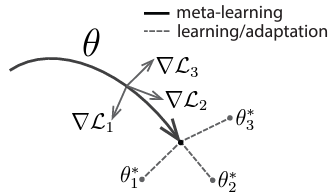
\includegraphics[width=0.6\textwidth]{figures/images/maml_weights.png}
    \caption{Diagram of MAML algorithm, which optimizes for a representation $\theta$ that can quickly adapt to new tasks}
    \label{fig:maml_weights}
\end{figure}

The MAML algorithm is the base for different methods which apply Few-Shot Imitation Learning in the context of Behavioral Cloning \cite{finn2017one_shot_visual_il,yu2018daml,yu2018one_shot_hil}.

In \cite{finn2017one_shot_visual_il}, MAML algorithm was used to prove the effectiveness of Meta-Learning in the context of real robot manipulation, with visual observations, as opposite to \cite{duan2017one_shot_il}. A Convolutional Neural Network was trained by following the Algorithm \ref{alg:maml}, using as loss-function the Mean Squared Error, computed between the predicted action and the ground truth one. For real-robot experiments a dataset of \textbf{1300} placing demonstrations (i.e., place an holded object in a target container), containing near to \textbf{100} different objects, was collected through teleportation. The trained system was tested by performing the adaptation step on one video demonstration, over 29 new objects, moreover, between the video demonstration and the actual execution, the objects configuration was changed. In this setting the system reached the $\mathbf{90\%}$ of success rate, outperforming baseline methods based on LSTM \cite{duan2017one_shot_il}, and contextual network (i.e., a Convolutional Neural Network that takes in input the current observation and the image representing the target state).

In \cite{yu2018daml}, the \textit{Domain Adaptive Meta-Learning} algorithm (DAML) was proposed with the goal of learning to infer a policy from a single human demonstration. To achieve it, a two-step algorithm was proposed. In the first-step, called \textbf{Meta-Learning step}, given in input, for each task $\mathcal{T}$, a set of human demo $\mathcal{D}^{h}_{\mathcal{T}}$ and a set or robot demo $\mathcal{D}^{r}_{\mathcal{T}}$ (Figure \ref{fig:daml_tasks}), the \textit{initial policy parameters} $\theta$ and the \textit{adaptive loss} parameters $\psi$ are learned, solving the problem in Formula \ref{eq:daml}.
\begin{equation}
 \label{eq:daml}
 \underset{\theta,\psi}{\min} \sum_{\mathcal{T} \sim p(\mathcal{T})} \sum_{\mathbf{d}^{h} \sim D^{h}_{\mathcal{T}}} \sum_{\mathbf{d}{^r} \sim D^{r}_{\mathcal{T}}} \mathcal{L}_{BC}(\theta - \alpha \nabla_\theta\mathcal{L}_{\psi}(\theta,\mathbf{d}^{h}), \mathbf{d}^{r})
\end{equation}

\newline The outer loss is the classic supervised Behavioral Cloning loss, defined as $\mathcal{L}_{BC}(\phi, \mathbf{d^{r}}) = \sum_{t} \log(\pi_{\phi}(a_{t} \mid s_{t}, o_{t}))$. The inner loss, $\mathcal{L}_{\psi}$, is a learned \textbf{adaptive loss}. Specifically, $\mathcal{L}_{\psi}$ is used during Meta-Adaptation, where the policy parameters are updated by evaluating the gradients derived from $\mathcal{L}_{\psi}$. This process involves using a video of a human demonstrating a new task $\mathcal{T}$ as input, leading to the policy update defined by $\phi_{\mathcal{T}} = \theta - \alpha \nabla_{\theta} \mathcal{L}_{\psi}(\theta, \mathbf{d}^{h})$. 
\newline This adaptive loss is the key component proposed in DAML. To use it effectively, it is necessary to learn the parameters $\psi$, observing how there is no direct correspondence between the human video demonstration and the robot's ground truth actions. To address this challenge, the authors of DAML observed that while the policy learns to produce appropriate actions through the $\mathcal{L}_{BC}$ loss, the adaptive loss should instead adjust the perceptual aspect of the policy, focusing on human motion and the manipulated object. Based on this insight, the authors implemented the function $\mathcal{L}_{\psi}$ using a 1D Temporal Convolutional Network (Figure \ref{fig:daml_temporal_adaptation_loss}). The convolutional layers are applied to a stack of embeddings generated by the policy $\pi$ across different frames of the video demonstrations. The parameters of this module are learned during the meta-training phase, following the weight update process described in Formula \ref{eq:daml_temporal_adaptation_loss}. The objective of $\mathcal{L}_{\psi}$ is to generate task-specific policy parameters $\phi_{\mathcal{T}}$ that guide the policy to produce effective actions.

\begin{equation}
 \label{eq:daml_temporal_adaptation_loss}
 \begin{matrix}
    (\theta, \psi) \leftarrow(\theta, \psi)-\beta \nabla_{\theta, \psi} \mathcal{L}_{\mathrm{BC}}\left(\phi_{\mathcal{T}}, \mathbf{d}^r\right) \\ \\
   \phi_{\mathcal{T}}=\theta-\alpha \nabla_\theta \mathcal{L}_\psi\left(\theta, \mathbf{d}^h\right)
   \end{matrix}
\end{equation}

\newline Experimental evaluation on tasks such as placing, pushing, and pick-and-place, has shown that: \begin{itemize}
    \item The system was able to generalize across both new objects and objects configuration starting from only a single human demonstration;
    \item A performance degradation was observed in large domain-shift experiments, such as novel backgrounds and different camera view-points.
\end{itemize}
\begin{figure}[t]
    \centering
    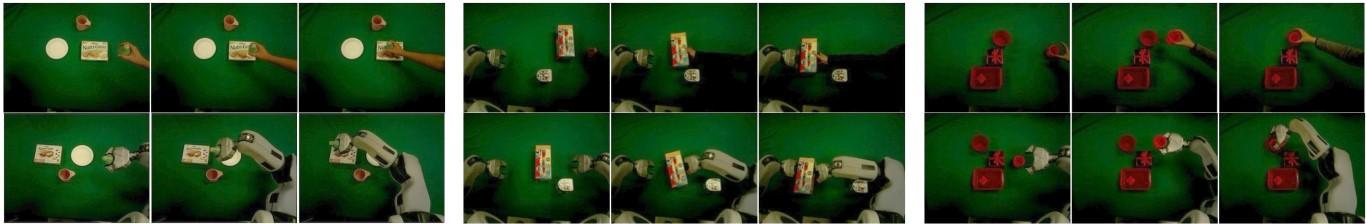
\includegraphics[width=\textwidth]{figures/images/daml/tasks.jpg}
    \caption{Tasks performed in \cite{yu2018daml}. (Top row) Human demonstration, (Bottom row) robot demonstration. (Left) Placing task, (Middle) pushing task, (Right) pick-and-place task.}
    \label{fig:daml_tasks}
\end{figure}

\begin{figure}[t]
    \centering
    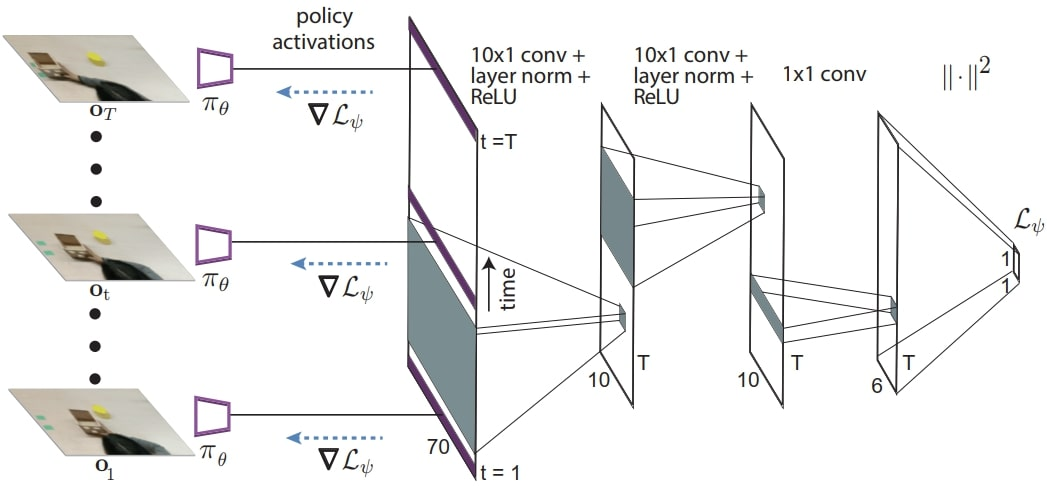
\includegraphics[width=0.8\textwidth]{figures/images/daml/daml_temporal_adaptation_loss.jpg}
    \caption{The Temporal Adaptation Loss architecture applies 1D temporal convolutional layers to the stacked embeddings generated by the policy $\pi$ from the frames of the human video demonstration.}
    \label{fig:daml_temporal_adaptation_loss}
\end{figure}

Meta-Learning algorithms have demonstrated intriguing properties, notably their capacity for few-shot generalization to novel objects and object configurations. However, it has been observed that during the adaptation step, these methods tend to lose their effectiveness in performing other tasks. This limitation has underscored the need for the development of Multi-Task Imitation Learning methods, which aim to address these shortcomings and enable more versatile task execution in complex scenarios. These kind of methods will be discussed in the following paragraphs.

\textbf{Zero-Shot MTIL} refers to approaches that aim to train a model capable of solving different tasks without any further adaptation or backpropagation steps. This approach addresses a key issue in Meta-Learning methods, which is the problem of forgetting how to solve previous tasks after adapting to a new one. The goal is to develop a single policy that can handle multiple tasks in a zero-shot manner.

In this context, a crucial design choice is how to convey the desired task to the policy. The literature identifies two main methods to address this problem:

\begin{enumerate}
    \item \textit{Language Conditioned}: These methods leverage natural language descriptions of tasks to inform the model about the task to be executed.
    \item \textit{Visual Conditioned}: These methods use visual information (e.g., goal-state images, video demonstrations) to provide the model with the task instructions.
\end{enumerate}
\textcolor{red}{ToDo}

\textit{Language Conditioned}

\textit{Visual Conditioned}